

\noindent\textbf{6.} Execute uma busca em profundidade a partir do vértice 0 no grafo orientado dado pelas listas de adjacência a seguir. Exiba o rastreamento da busca.\\[6pt]
\noindent0: 1 4\\
1: 2 5\\
2: 3\\
3: 7\\
4: 8\\
5: 4\\
6: 5 10 2\\
7: 11 6\\
8: 9\\
9: 5 8\\
10: 9\\
11: 10\\

\textbf{Resposta:} A figura \ref{fig:7.6-1} mostra o grafo formado pela lista de adjacências dada, bem como o rastreamento no momento em que o vértice 3, 6 e 8 são descobertos, e o resultado final da \proc{DFS} ao final de todas as chamadas recursivas, respectivamente. Os tempos $d$ e $f$ estão no vetor à direita e, também, acima de cada vértice.

\begin{center}
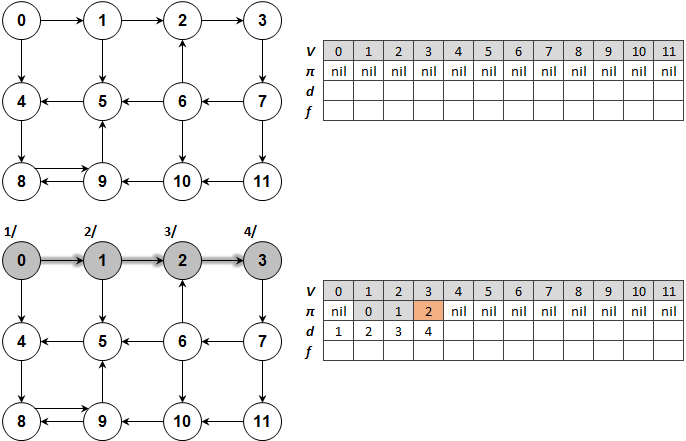
\includegraphics[width=0.9\textwidth]{q7-06-p1.png}
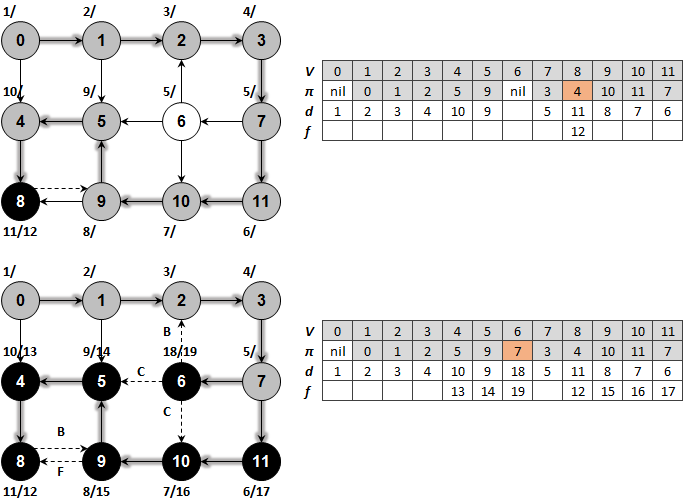
\includegraphics[width=0.9\textwidth]{q7-06-p2.png}
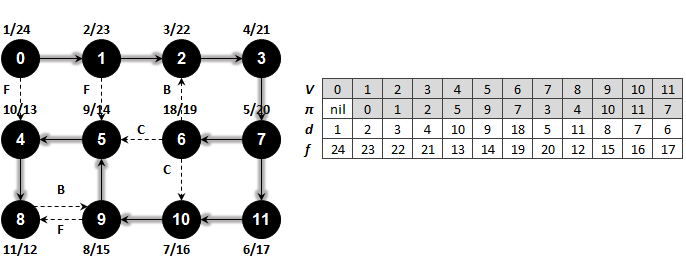
\includegraphics[width=0.9\textwidth]{q7-06-p3.png}
\captionof{figure}{Rastreamento da \proc{DFS} na lista de adjacências dada.}
\label{fig:7.6-1}
\end{center}